\documentclass[12pt,twoside]{report}
\usepackage[utf8]{inputenc}
\usepackage{graphicx}
\graphicspath{ {images/} }
\usepackage{caption}
\usepackage{subcaption}
\usepackage[a4paper,width=150mm,top=25mm,bottom=25mm,bindingoffset=6mm]{geometry}
\usepackage{fancyhdr}
\pagestyle{fancy}
\fancyhead{}
\fancyhead[RO,LE]{Modelling and Solving the Vehicle Routing Problem (VRP)}
\fancyfoot{}
\fancyfoot[LE,RO]{\thepage}
\fancyfoot[LO,CE]{Chapter \thechapter}
\fancyfoot[CO,RE]{Mario Sessa}
\renewcommand{\headrulewidth}{0.4pt}
\renewcommand{\footrulewidth}{0.4pt}
\usepackage{tikz}
\usetikzlibrary{fit, positioning}
\usepackage{lipsum}
\usepackage{hyperref}
\bibliographystyle{ieeetr}
\usepackage{biblatex}
\addbibresource{references.bib}


\begin{document}

\begin{titlepage}
    \begin{center}
        \vspace*{0.1cm}
        
          
        
\includegraphics[width=0.6\textwidth]{images/logo-unibo.png}
        
        \large
         \textbf{Department of Computer Science}
         \vspace{0.5cm}
         
         \textbf{Exam of Decision Making \& Constraint Programming\newline   
         Project Report}
         \vspace{1cm}
         
         Academic Year 2020 - 2021
         
         
         \vspace{2cm}
        
        
        \LARGE
        \textbf{Modelling and Solving the Vehicle Routing Problem (VRP)}
        
        
        \vspace{1.5cm}
        \large
        \textbf{Mario Sessa}
        
        0000983529
        
       % \vfill
        \vspace{1.5cm}
        A project report of modelling and solving the Vehicle Routing Problem using the Constraint Programming approach

        
        \vspace{0.8cm}
      \begin{flushright}
        \footnotesize
        Alma Mater Studiorum, University of Bologna \\
        Department of Computer Science\\
        Bologna\\
        Via Zamboni, 33, 40126\\
        Italy \\
        \end{flushright}
        
    \end{center}
\end{titlepage}


\tableofcontents

\chapter{Introduction}
\section{Problem Presentation}
The Vehicle Routing Problem (VRP) is an NP-optimization problem that has been of great interest for decades for both, science and industry. We got an example with Amazon that use it for the management of the deliveries from his orders around the world. The aim of our version of VRP is to find a set of minimum total cost routes for a fleet of capacitated vehicles (CVRP) based at a single depot, to serve a set of customers under the following constraints:
\begin{enumerate}
    \item each route must begin and ends at the depot node
    \item each customer/location is visited exactly once
    \item the total demand of each routes does not exceed the capacity of vehicle assigned to the route
\end{enumerate}
This type of problem is referred to a combination of two sub-problem:
\begin{enumerate}
    \item Travelling Salesman Problem (TSP) which define an Hamiltonian routes similar to the combined routes of the Vehicle Routing Problem
    \item Knapsack Problem which define constraints to manage the capacities of the vehicles in respect of the customers demands of their routes
\end{enumerate}
The VRP belongs to the category of NP-hard problems that can be exactly solved only for small instances of the problem. Therefore, many researchers have concentrated on developing heuristics algorithm to solve this problem for hard instances or find a good solution (not necessarily the optimal one). In the following section, we will explain the strategy used to solve it using a Constraint Programming approach.
\newpage
\section{Formal Problem Definition}
Let G = (V,H) be a complete directed graph with \begin{math}V \end{math} on domain \begin{math} \{1,2,3,...n, n + 1\} \end{math} as the set of nodes and H = \begin{math}\{(i,j) : i,j \in V, i \neq j\end{math}\} a set of arcs, where node n + 1 represents the depot for a fleet of v vehicles with capacities \begin{math}C_{w} > 0, w \in \{1,2..v\} \end{math}. The remaining n nodes represents the geographically position of customers. Each node of V has a location with coordinates \begin{math}(x_{i}, y_{i}) \end{math} for a node \begin{math}i \in \{1,2,3,.., n + 1\}\end{math}. Each customer \begin{math} c \in V - \{n-1\}\end{math} has a demand \begin{math} 0 < de_{c} \leq \sum_{w = 1}^{v} C_{w}.\end{math} We also have a set of distances \begin{math} D = \{d_{ij} | i,j \in V\} \end{math} represents the weight of the edge between nodes i and j.
\newline \newline Each vehicle needs to start and end his route to the depot, every customer can be visited just from a vehicle. Moreover, given \begin{math}de_{cw}\end{math} the demand \begin{math} d_{c}\end{math} satisfied by a vehicle \begin{math}w \in \{1,2...v\},\sum_{i,j \in V }d_{cw} \leq C_{w}, \forall w \in \{1,2...v\}\end{math}. \newline \newline Defined \begin{math}d_{ijw}\end{math} the distance traveled by a vehicle w and \begin{math} b_{w} \in \{0,1\}\end{math} a boolean representing if a vehicle is used or not, the aim of the problem is to minimize \begin{math}\sum_{w \in \{1,2..v\}}d_{ijw} + (\sum_{w \in \{1,2..v\}}b_{w}) * weight_{v}\end{math} with \begin{math}weight_{v}\end{math} is a constant value to balance the optimal result between the use of vehicles and the total distance traveled. [1]\newline
\newline\newline


\begin{figure}[h]
    \centering
    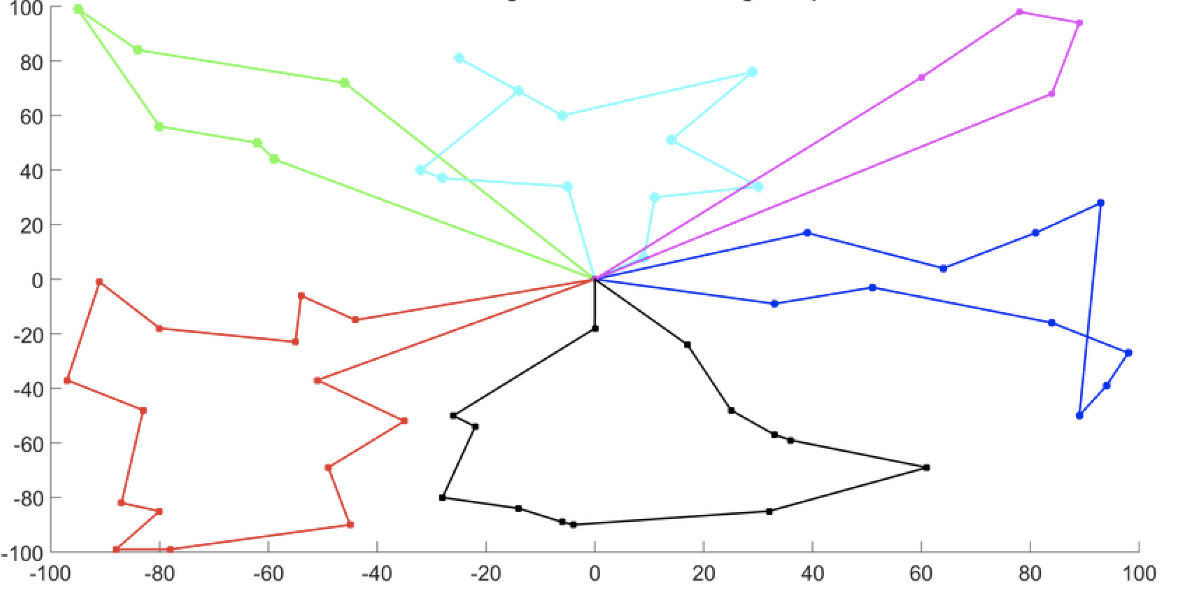
\includegraphics[width=1.0\textwidth]{images/vrp-graph.png}
    \caption{Graph of a VRP solution based on the use of 6 vehicles}
    \label{fig:mesh1}
\end{figure}

\chapter{Modelling VRP in Constraint Programming}
\section{Input Data and any Potential Data Processing}
Let N the number of customers, input data are as follow:
\begin{enumerate}
    \item \begin{math}locX_{i}\end{math} for each i in \{1..N+1\} with a float domain defines the coordinate X of a location \begin{math}L_{i}\end{math}, the last one is a reference of the depot coordinate 
    \item \begin{math}locY_{i}\end{math} for each i in \{1..N+1\} with a float domain defines the coordinate Y of a location, the last one is a reference of the depot coordinate
    \item a list \begin{math}(de_{1}, ..., de_{N})\end{math} with \begin{math}d_{i}, i \in \{1..N\}\end{math} the demand of the customer i
    \item V is the number of vehicles available
    \item a list \begin{math}(c_{1},..., c_{V})\end{math} with \begin{math} c_{i}, i \in \{1..V\}\end{math} the capacity of the vehicle i
\end{enumerate}
From this set of input data we can define following processing data, useful to establish constraints in the model:
\begin{enumerate}
    \item 
\section{Decision Variables}
\section{Problem \& Additional Constraints}
\subsection{Main Constraints}
\subsection{Additional Constraints}
\section{Objective Function}



\chapter{Experimental Study}
\section{Experimental Setup}
\subsection{Software and Hardware}
The model was implied using a constraint programming language: MiniZinc 2.5.3. The solver associated is Gecode 6.3.0. Experiments were done on a Macbook Pro 2018 with processor at 2,2 GHz, 6-Core on a Intel Core i7 of 9th generation and a memory of 16 GB, 2400 Mhz DDR4.
\subsection{Instances}
The following table represents instances with their features referred to the number of customers, the number of vehicles, the total capacity available to satisfy the customers demands and the total customers demands. Total capacity and total demands are distributed unevenly between customers and vehicles respectively.
\begin{table}[!h]
\label{T:instances}
\begin{center}
\begin{tabular}{| c | c | c | c | c | }
\hline
\textbf{Instance} & \multicolumn{4}{ c |}{\textbf{Features}}  \\ 
\cline{2-5}
& \textbf{\#Customers} & \textbf{\#Vehicles} & \textbf{Tot. Capacity} & \textbf{Tot. Demand}  \\
\hline
% Table values
PR01 & 47 &  4  &  800 & 647 \\ \hline
PR02 & 95 & 20  & 3,900 & 1,210\\ \hline
PR03 & 143 &  20 & 3,800 & 1,765\\ \hline
PR04 & 191 & 20  & 3,700 & 2,472\\ \hline
PR05 & 239 & 20 & 3,600 & 3,335\\ \hline
PR06 & 287 & 20 & 3,700 & 3,665\\ \hline
PR07 & 71 & 20  & 4,000 & 928\\ \hline
PR08 & 143 & 20 & 3,800 & 1,985\\ \hline
PR09 & 215 & 20 & 3,600 & 2,735\\ \hline
PR10 & 287 & 20 & 3,900 & 3,825\\ \hline
PR11 & 47 & 20 & 4,000 & 647\\ \hline \hline

\end{tabular}
\end{center}
\end{table}
\newpage
\subsection{Search Strategy}
[2] The following list represents the search strategy associated with their acronyms carried out on the model in Minizinc with Gecode solver:
\begin{enumerate}
    \item \textbf{SEQDR}: identify the sequential search structured in the following ordered sequence:
    \begin{enumerate}
        \item Take a decision for each element of the vehicles list \begin{math} ve \end{math} using domWdeg and random value heuristics
        \item Take a decision for each element of successors list \begin{math} s \end{math} using domWdeg and random value heuristics
    \end{enumerate} with the Luby Strategy on L = 250
    \item \textbf{SEQSM}: identify the sequential search structured in the following ordered sequence:
    \begin{enumerate}
        \item Take a decision for each element of the vehicles list \begin{math} ve \end{math} using smallest domain and minimum value heuristics
        \item Take a decision for each element of the successors list \begin{math} s \end{math} using domWdeg and random value heuristics
        \end{enumerate} with the Luby Strategy on L = 300.
    \item \textbf{DRLSN}: identify the search structured with domWdeg and random domain heuristic on \begin{math} s \end{math} variables list using Luby Strategy with L = 350 and the Large Neighbourhood Strategy fixing 85\% of the \begin{math}s\end{math} variables list.
    \item \textbf{SMLNS}: identify the SEQ heuristics using Large Neighbourhood Strategy fixing 85\% of the \begin{math} s \end{math} variables list.
    
    
\end{enumerate}
\newpage
\section{Experimental Results}
\subsection{Tables of Results}
\begin{itemize}
    \item Table of Failures
    
        \begin{table}[!h]
    \label{T:instances}
        \begin{center}
        \begin{tabular}{| c | c | c | c | c | c | c | c | c | }
\hline

\textbf{Instance} & \textbf{SEQDR} & \textbf{SEQSM} & \textbf{DRLNS} & \textbf{SMLNS}  \\
\hline
% Failures table
PR01 & 1,617,823  & 1,846,879 &  1,758,637 & 1,790,778\\ \hline
PR02 & 261,731  & 276,031  &  304,075 & 307,405  \\ \hline
PR03 & 107,615  & 111,227 &  108,265 & 153,923 \\ \hline
PR04 & 54,289  & 59,572 &  53,443 & 86,818  \\ \hline
PR05 & 25,276  & 35,984 &  30,839 & 52,607  \\ \hline
PR06 & 14,075  & 24,078 & 15,912 & 37,785 \\ \hline
PR07 & 365,984  & 431,475 &  397,412 & 523,065  \\ \hline
PR08 & 101,392  & 104,439 &  107,554 & 168,311  \\ \hline
PR09 & 32,350  & 31,886 &  33,942 & 69,721  \\ \hline
PR10 & 13,015  & 15,580  &  14,493 & 36,780  \\ \hline
PR11 & 738,268  & 491,894 &  650,122 & 723,032  \\ \hline
\hline
\end{tabular}
\end{center}
\end{table}

    \item Table of Optimal Solutions
        \begin{table}[!h]
    \label{T:instances}
        \begin{center}
        \begin{tabular}{| c | c | c | c | c | c | c | c | c | }
\hline

\textbf{Instance} & \multicolumn{2}{ c |}{\textbf{SEQDR}} & \multicolumn{2}{ c |}{\textbf{SEQSM}} & \multicolumn{2}{ c |}{\textbf{DRLNS}} & \multicolumn{2}{ c |}{\textbf{SMLNS}}   \\
\cline{2-3}  \cline{4-5} \cline{6-7} \cline{8-9}
& \textbf{Dist.} & \textbf{Veh.} & \textbf{Dist.} &\textbf{Veh.} & \textbf{Dist.} & \textbf{Veh.} & \textbf{Dist.} & \textbf{Veh.}  \\
\hline
% Table values
PR01 & 2,395,540  & \textbf{4} &  2,300,229 & \textbf{4} & 940,728 & \textbf{3} & 959,341  & \textbf{3}  \\ \hline
PR02 & 5,759,370  & \textbf{20} &  5,171,574 & \textbf{7} & 2,481,414 & \textbf{9} & 2,280,093  & \textbf{9}  \\ \hline
PR03 & 1,1090,848  & \textbf{20} &  10,433,132 & \textbf{10} & - & \textbf{-} & 6,768,854  & \textbf{10}  \\ \hline
PR04 & 12,834,190  & \textbf{20} &  12,666,579 & \textbf{14} & - & \textbf{-} & 8,538,335  & \textbf{14}  \\ \hline
PR05 & 13,939,739  & \textbf{20} & 13,457,287 & \textbf{19} & - & \textbf{-} & 9,538,436  & \textbf{19}  \\ \hline
PR06 & 18,746,215  & \textbf{20} &  19,188,412 & \textbf{20} & - & \textbf{-} & 14,869,127  & \textbf{20}  \\ \hline
PR07 & 5,040,291  & \textbf{20} &  4,238,722 & \textbf{5} & 1,227,767 & \textbf{7} & 1,265,506  & \textbf{4}  \\ \hline
PR08 & 10,159,608  & \textbf{20} &  9,736,174 & \textbf{11} & - & \textbf{-} & 5,649,437  & \textbf{11}  \\ \hline
PR09 & 15,267,652  & \textbf{20} &  15,056,711 & \textbf{16} & - & \textbf{-} & 10,050,036  & \textbf{16}  \\ \hline
PR10 & 19,773,277  & \textbf{20} & 19,778,614  & \textbf{20} & - & \textbf{-} & 13,794,840  & \textbf{20}  \\ \hline
PR11 & 3,171,559  & \textbf{18} &  2,413,564 & \textbf{4} & 920,830 & \textbf{3} & 913,719  & \textbf{3}  \\ \hline
\hline
\end{tabular}
\end{center}
\end{table}
\newline
The previous table have reported the number of the total distance traveled on the combined route (\begin{math} 
Dist. \equiv td\end{math}) and the number of vehicles used (\begin{math}Veh. \equiv vu\end{math}). The objective value \begin{math} min(f(td,vu)) \end{math} have been calculated using the objective function, \begin{math} tu \end{math} and \begin{math} vu \end{math} defined in the paragraph 2.4. and \begin{math} w = 1000 \end{math}.
\end{itemize}
\newpage

\chapter{Conclusions}
We have described a version of the Capacitated Vehicle Routing Problem with Constraint Programming method. The nature of problem is reducible to the combination between Travelling Salesman and Knapsack Problem. We have considered the \begin{math} circuit \end{math} global constraint to define the Hamiltonian property given by the Travelling Salesman modelling and the capacity symmetry breaking constraint from the Knapsack model. Furthermore, the model has been improved by an implied \begin{math}alldifferent\end{math} constraint. Finally, the search strategies have had problems in finding optimal solutions for instances with more than 100 customers. Moreover, they have been efficient in sequential cases and adding the Large Neighbourhood Strategy has given better results than the complete approach. 



\begin{thebibliography}{9}

\bibitem{travelling-salesman-problem} 
Travelling Salesman Problem Definition,
\\\texttt{https://en.wikipedia.org/wiki/Travelling\_salesman\_problem}


\bibitem{knapsack-problem}
Knapsack Problem Definition
\\\texttt{https://en.wikipedia.org/wiki/Knapsack\_problem}
\end{thebibliography}

\end{document}

\begin{thebibliography}{9}
\bibitem{latexcompanion} 
Michel Goossens, Frank Mittelbach, and Alexander Samarin. 
\textit{The \LaTeX\ Companion}. 
Addison-Wesley, Reading, Massachusetts, 1993.

\bibitem{einstein} 
Albert Einstein. 
\textit{Zur Elektrodynamik bewegter K{\"o}rper}. (German) 
[\textit{On the electrodynamics of moving bodies}]. 
Annalen der Physik, 322(10):891–921, 1905.

\bibitem{travelling-sales-man-problem} 
Travelling Salesman Problem Definition
\\\texttt{https://en.wikipedia.org/wiki/Travelling\_salesman\_problem}

\bibitem{knapsack-problem}
Knapsack Problem Definition
\\\texttt{https://en.wikipedia.org/wiki/Knapsack_problem}

\end{thebibliography}